% 3. Veb aplikacija EduGrader
\chapter{Veb aplikacija EduGrader}
\label{sec:aplikacija}

EduGrader je veb aplikacija za automatsko ocenjivanje odgovora otvorenog tipa sa studentskih ispita pomoću velikih jezičkih modela.
To je deo sistema namenjen upotrebi u nastavi, organizovan u tri sloja (slika~\ref{fig:architecture}):

\begin{itemize}
    \item \textbf{Klijentski sloj.} Jednostranična aplikacija (engl. \emph{single-page application}, SPA)
    izgrađena u tehnologijama React~19 i TypeScript, koju poslužuje Nginx server.
    Prikazi za nastavnike i studente su odvojeni: nastavnici upravljaju kursevima,
    testovima i pitanjima i pregledaju rešene testove, a studenti rešavaju testove i prate svoje rezultate.
    Na prikazu rešenog testa, uz svaki odgovor stoje i ocena nastavnika i ocena koju je predložio jezički model; konačnu odluku donosi nastavnik.
    Autentifikacija se obavlja putem JWT-a (engl. \emph{JSON Web Token}) sa kontrolom pristupa zasnovanom na ulogama.
    \item \textbf{Serverski sloj.} REST (engl. \emph{representational state transfer}) API izgrađen u tehnologijama Python~3,
    Django~5.1 i Django REST Framework.
    Izlaže CRUD (engl. \emph{create, read, update, delete}) operacije nad domenskim modelima
    i sadrži modul za ocenjivanje, odgovoran za sastavljanje promptova, pozivanje modela,
    izdvajanje ocene iz odgovora i trajno čuvanje rezultata.
    \item \textbf{Sloj baze podataka.} Realizovan kroz Django ORM (engl. \emph{object-relational mapping})
    nad bazom SQLite,
    sa entitetima za kurseve, testove, pitanja, studentske odgovore i ocene.
    SQLite je izabran kao razvojna i prototipska baza, dovoljna za lokalno pokretanje:
    umesto zasebnog serverskog procesa, biblioteka SQLite radi u samom procesu aplikacije,
    a celu bazu čuva u jednoj datoteci.
    Django ORM dopušta prelazak na serverski sistem za upravljanje bazom (npr. PostgreSQL)
    izmenom konfiguracije, bez izmena u kodu aplikacije.
    Pored samih ocena čuvaju se i povratne informacije, promptovi i metapodaci, potrebni za kasnije analize.
\end{itemize}

Logika ocenjivanja i ponašanje modela razvijaju se nezavisno od korisničkog interfejsa;
klijentski i serverski deo komuniciraju samo preko REST API-ja.
Slika prikazuje i evaluacioni \emph{pipeline} u sistemu DVC (engl. \emph{Data Version Control})\footnote{\url{https://dvc.org}},
opisan u poglavlju~\ref{sec:pipeline}, koji koristi isti integracioni sloj.

% --- DIJAGRAM ARHITEKTURE (TikZ) ---
\begin{figure}[htbp]
\centering
\resizebox{\textwidth}{!}{%
\begin{tikzpicture}[
    node distance=0.6cm and 0.8cm,
    box/.style={draw, rounded corners=3pt, minimum height=0.9cm, text centered, font=\small},
    arr/.style={-{Stealth[length=2.5mm]}, thick},
    darr/.style={-{Stealth[length=2.5mm]}, thick, densely dashed},
    lbl/.style={font=\scriptsize, midway, fill=white, inner sep=1pt},
]

% ---- Klijentski sloj ----
\node[box, fill=red!8, minimum width=4.8cm, minimum height=1.6cm] (fe) {};
\node[font=\small\bfseries, anchor=north] at (fe.north) {Klijentski sloj};
\node[font=\scriptsize, anchor=south] at (fe.south) {React 19 + TypeScript};
\node[font=\scriptsize] at (fe.center) {Interfejs za ocenjivanje \textbar{} JWT};

% ---- Serverski sloj ----
\node[box, fill=red!8, minimum width=6.2cm, minimum height=3.4cm, right=2.2cm of fe] (be) {};
\node[font=\small\bfseries, anchor=north] at (be.north) {Serverski sloj};
\node[font=\scriptsize, anchor=north, yshift=-3mm] at (be.north) {Django 5.1 + Django REST Framework};

% Unutrašnje komponente
\node[box, fill=red!15, minimum width=4.4cm, font=\scriptsize] at ([yshift=-2mm]be.center) (gm) {Modul za ocenjivanje};
\node[box, fill=red!22, minimum width=4.4cm, font=\scriptsize, below=0.3cm of gm] (factory) {Fabrika integracija jezičkih modela};

% ---- Baza podataka ----
\node[box, fill=yellow!15, minimum width=2.8cm, minimum height=1.2cm, below=1.4cm of be] (db) {};
\node[font=\small\bfseries] at ([yshift=1.5mm]db.center) {Baza podataka};
\node[font=\scriptsize] at ([yshift=-3mm]db.center) {SQLite: kursevi, testovi, ocene};

% ---- LLM API-ji ----
\node[box, fill=red!8, minimum width=3.4cm, minimum height=1.1cm, align=center, right=2.2cm of factory, yshift=1.4cm]
  (openai) {\scriptsize OpenAI API\\[-1pt]\tiny gpt-4o-mini, gpt-4o, gpt-5};

\node[box, fill=red!8, minimum width=3.4cm, minimum height=1.1cm, align=center, right=2.2cm of factory]
  (deepseek) {\scriptsize DeepSeek API\\[-1pt]\tiny deepseek-chat, deepseek-reasoner};

\node[box, fill=red!8, minimum width=3.4cm, minimum height=1.1cm, align=center, right=2.2cm of factory, yshift=-1.4cm]
  (gemini) {\scriptsize Gemini API\\[-1pt]\tiny gemini-2.5-flash};

% ---- DVC pipeline ----
\node[box, fill=purple!8, minimum width=4.8cm, minimum height=1.6cm, below=1.4cm of fe] (pipe) {};
\node[font=\small\bfseries, anchor=north] at (pipe.north) {DVC \emph{pipeline}};
\node[font=\scriptsize] at (pipe.center) {Grupni eksperimenti};
\node[font=\scriptsize, anchor=south] at (pipe.south) {spajanje \textrightarrow{} ocenjivanje};

% ---- Strelice ----
\draw[arr] (fe.east) -- node[lbl, above] {REST API} (be.west |- fe.east);
\draw[arr] (be.south) -- node[lbl, right] {ORM} (db.north);
\draw[arr] (factory.east) -- ++(0.6,0) |- (openai.west);
\draw[arr] (factory.east) -- ++(0.6,0) |- (deepseek.west);
\draw[arr] (factory.east) -- ++(0.6,0) |- (gemini.west);
\draw[darr] (pipe.east) -- ++(0.8,0) |- node[lbl, below, pos=0.25] {koristi} (factory.west);

\end{tikzpicture}%
}
\caption{Arhitektura sistema EduGrader.
Klijentski sloj komunicira sa serverskim slojem preko REST API-ja.
Serverski sloj pristupa jezičkim modelima kroz jedinstven integracioni sloj (projektni obrazac fabrika) koji apstrahuje API-je pojedinačnih provajdera.
Sistem za automatizovanu evaluaciju (poglavlje~\ref{sec:pipeline}) koristi isti integracioni sloj za grupne eksperimente.
Integracija Gemini nije korišćena u eksperimentima opisanim u ovom radu.}
\label{fig:architecture}
\end{figure}

\section{Klijentska aplikacija}
\label{sec:webapp}

Klijentska aplikacija je jednostranična aplikacija koja koristi biblioteku React (verzija 19) i jezik TypeScript,
uz Vite kao alat za izgradnju i razvojno okruženje.
Rutiranje je rešeno bibliotekom React Router, kroz koju je aplikacija podeljena na dva modula sa odvojenim pravima pristupa:

\begin{itemize}
    \item \textbf{Nastavnički modul} omogućava pregled predmeta, kreiranje testova i pitanja i pregled rešenih studentskih testova,
    sa prikazom nastavničke ocene uz predlog ocene jezičkog modela za svaki odgovor.
    \item \textbf{Studentski modul} omogućava pregled nadolazećih testova, izradu testa i uvid u rezultate već urađenih testova.
\end{itemize}

Slike~\ref{fig:ui-kurs}--\ref{fig:ui-student} prikazuju tipičan tok rada.
Nastavnik na stranici kursa unosi pitanja sa referentnim odgovorima i od njih sastavlja testove (slika~\ref{fig:ui-kurs}).
Kada student preda test (slika~\ref{fig:ui-student}),
nastavnik pri pregledu za svaki odgovor vidi predlog ocene jezičkog modela i, po potrebi, njegovo obrazloženje,
a konačnu ocenu unosi sam (slika~\ref{fig:ui-ocena}).
Predlog modela je tako samo polazna tačka: nastavnik ga može prihvatiti ili prepraviti, što je princip iz uvoda da je čovek sastavni deo sistema.

Elementi interfejsa su na engleskom, dok su pitanja, referentni odgovori i studentski odgovori na srpskom,
isto kao u eksperimentima iz poglavlja~\ref{sec:rezultati}.

\begin{figure}[htbp]
\centering
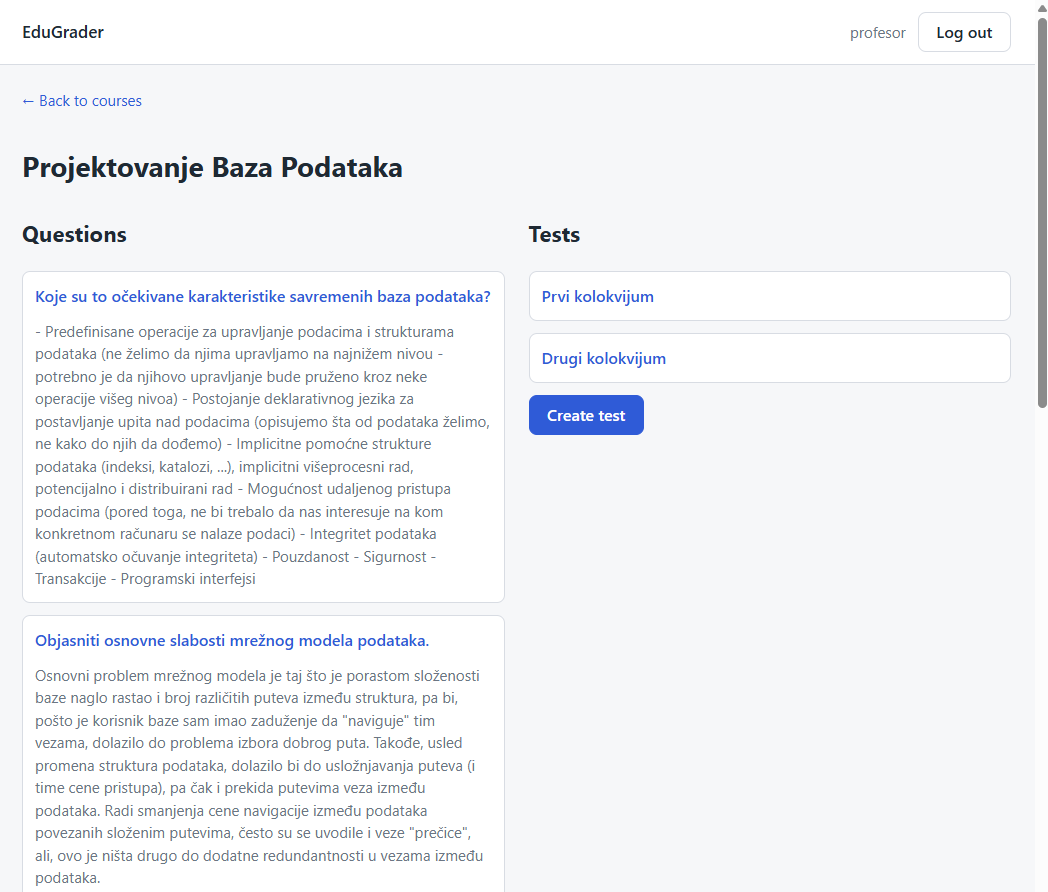
\includegraphics[width=0.8\textwidth]{screenshots/profesor_course.png}
\caption{Nastavnički modul: stranica kursa sa pitanjima, njihovim referentnim odgovorima i listom testova.}
\label{fig:ui-kurs}
\end{figure}

\begin{figure}[htbp]
\centering
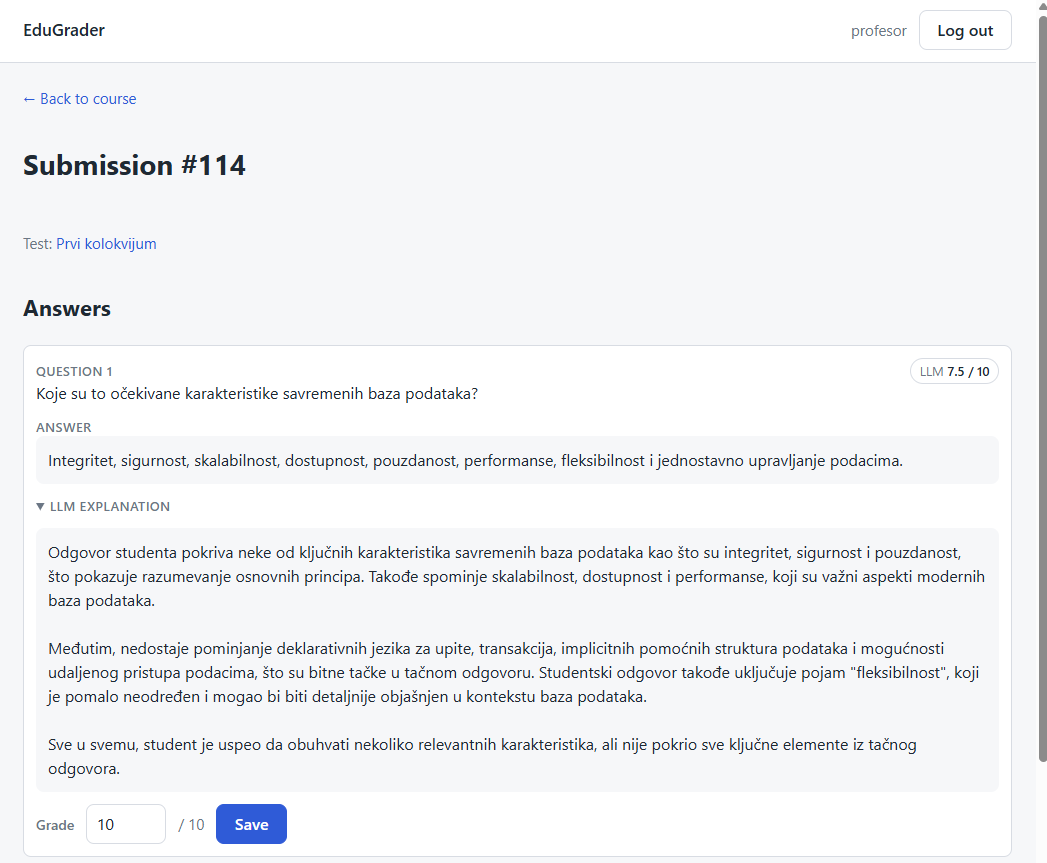
\includegraphics[width=0.8\textwidth]{screenshots/professor_test_submittion_with_llm.png}
\caption{Nastavnički modul: pregled rešenog testa.
Uz svaki odgovor prikazan je predlog ocene jezičkog modela (ovde 7,5 od 10) sa rasklopljenim obrazloženjem,
a konačnu ocenu unosi nastavnik u polje \emph{Grade}.
Na snimku je nastavnik, uprkos predlogu modela od 7,5, uneo konačnu ocenu 10,
što ilustruje da konačna odluka ostaje na njemu.}
\label{fig:ui-ocena}
\end{figure}

\begin{figure}[htbp]
\centering
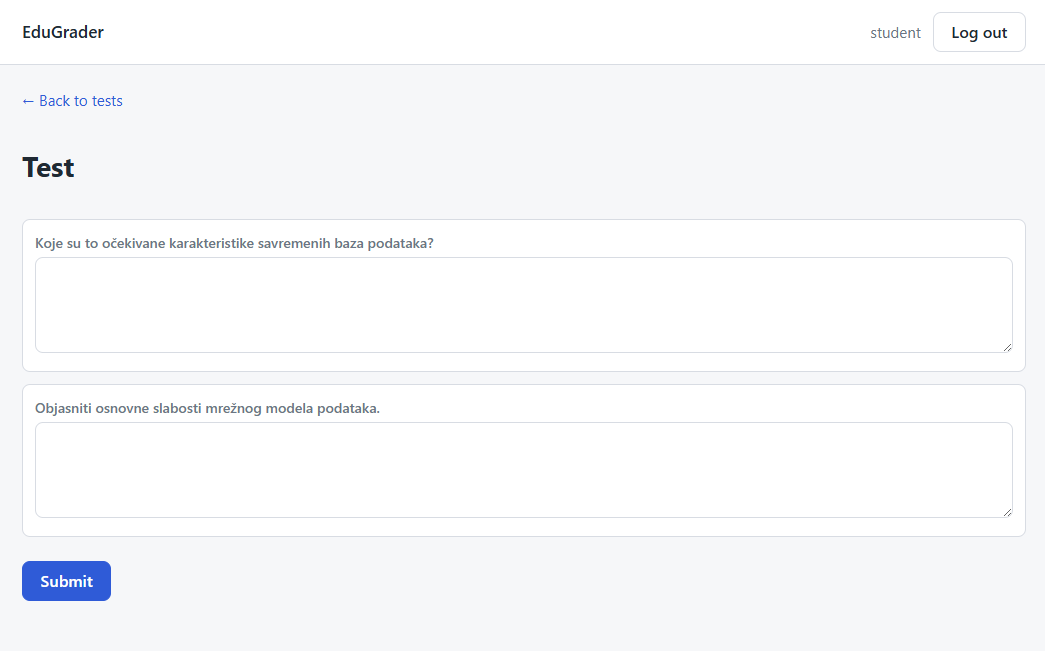
\includegraphics[width=0.8\textwidth]{screenshots/student_test.png}
\caption{Studentski modul: izrada testa.}
\label{fig:ui-student}
\end{figure}

Grupno ocenjivanje se u trenutnoj implementaciji ne pokreće iz korisničkog interfejsa:
logika ocenjivanja izložena je kao funkcije serverskog modula za ocenjivanje,
a eksperimenti opisani u poglavlju~\ref{sec:pipeline} pokreću je kroz \emph{pipeline} u sistemu DVC,
nad podacima pripremljenim u vidu CSV (engl. \emph{comma-separated values}) datoteka.
Izbor modela, režima ocenjivanja i konfiguracije strogosti zadaje se kroz parametarske datoteke tog \emph{pipeline}-a, a ne kroz veb interfejs.

Autentifikacija koristi JWT, koji se čuva u skladištu sesije (engl. \emph{session storage}) pregledača, koje traje dok je kartica otvorena.
Uloge (nastavnik ili student) ugrađene su u njega i na osnovu njih se sprovodi kontrola pristupa rutama.
U razvojnom okruženju Vite server prosleđuje API pozive ka serverskom delu,
dok se u produkciji statička verzija aplikacije poslužuje kroz Nginx.

\section{Serverska aplikacija}

Serverski deo je Django projekat podeljen na tri aplikacije, u skladu sa Django konvencijom razdvajanja odgovornosti:

\begin{itemize}
    \item \textbf{Aplikacija za autentifikaciju} implementira prilagođeni korisnički model sa ulogama student i nastavnik,
    izdavanje i osvežavanje JWT-a,
    kao i klase dozvola (engl. \emph{permission classes}) kojima se pojedinačni API pozivi ograničavaju na odgovarajuću ulogu.
    \item \textbf{Glavna aplikacija} definiše domenske modele, kurs, pitanje,
    test, studentski test i studentski odgovor,
    zajedno sa serijalizatorima i CRUD \emph{endpoint}-ima, adresama REST API-ja preko kojih se izvode pojedinačne operacije nad njima.
    Studentski odgovor čuva i ocenu koju je dodelio nastavnik, što omogućava kasnije poređenje sa ocenama modela.
    \item \textbf{Aplikacija za ocenjivanje} sadrži logiku ocenjivanja i integracije sa jezičkim modelima.
    Za svaki ocenjeni odgovor kreira zapis sa korišćenim promptom, instrukcijama,
    kompletnim odgovorom modela i izdvojenom numeričkom ocenom, pa je svaka ocena naknadno proverljiva.
\end{itemize}

Sistem je zapakovan u Docker kontejnere: jedan kontejner izvršava Django aplikaciju,
a drugi Nginx koji poslužuje klijentsku aplikaciju i prosleđuje API saobraćaj.

\section{Integracija jezičkih modela}
\label{sec:integracije}

Jezičkim modelima pristupa se isključivo preko API-ja provajdera u oblaku;
nijedan model se ne izvršava lokalno.
Više provajdera pokriveno je projektnim obrascem fabrika (engl. \emph{factory}),
sa apstraktnim interfejsom \texttt{LLMIntegration} i metodom \texttt{prompt()} čiji su parametri ulazni tekst,
identifikator modela, sistemske instrukcije i temperatura.
Metoda vraća par: izdvojeni tekstualni odgovor i kompletan odgovor API-ja, koji se čuva radi sledivosti.

Implementirane su tri integracije, kao tri implementacije zajedničkog interfejsa
(\texttt{LLMIntegration}), dostupne istovremeno i birane po simboličkom imenu:

\begin{itemize}
    \item \textbf{OpenAI}, koristi zvanični OpenAI Python SDK (engl. \emph{software development kit}).
    Podržani modeli: \texttt{gpt-\allowbreak 4o-\allowbreak mini}, \texttt{gpt-4o} i \texttt{gpt-5}.
    \item \textbf{DeepSeek}, koristi OpenAI-kompatibilni API \emph{endpoint} preko istog SDK-a, sa promenjenom baznom adresom.
    Podržani modeli: \texttt{deepseek-chat} (V3) i \texttt{deepseek-reasoner} (R1).
    \item \textbf{Google Gemini}, koristi zvanični Google GenAI Python SDK.
    Podrazumevani model: \texttt{gemini-2.5-flash}.
    U aplikaciji služi za generisanje simuliranih studentskih odgovora pri testiranju
    i nije korišćena u eksperimentima opisanim u ovom radu.
\end{itemize}

Fabrička funkcija instancira odgovarajuću klasu na osnovu simboličkog imena integracije
(\texttt{openai}, \texttt{deepseek}, \texttt{gemini}).
Nov provajder se tako dodaje implementacijom jedne klase, bez izmena u logici ocenjivanja;
isti mehanizam koriste i veb aplikacija i sistem za automatizovanu evaluaciju iz poglavlja~\ref{sec:pipeline}.
API ključevi čuvaju se kao promenljive okruženja i nikada nisu ugrađeni u izvorni kod.
